\clearpage
\chapter{Introduction}
\label{ch:intro}

As robots continue to become more integrated into our daily lives, researchers are working to improve human-robot interaction \cite{premaratne2014human}. Gesture recognition technology has emerged as a key tool for enabling more natural interactions with robots, replacing traditional human-machine interfaces like keyboards, mice, and joysticks \cite{smith2022hand}. This~application can be a good intervention for people with disabilities. By using hand gestures, they can more easily interact with virtual environments, robotics, home automation, clinical operations, game controls, desktop/tablet applications, delivery services, sign language, and more. 


Drones are remotely controlled robots can be operated via a remote control device or~a~smartphone. They're a popular tool in many of these applications, often used for sports event coverage, aerial photography, and emergency response. Developing automatic systems that can recognize hand gestures would greatly improve the ability to interact with drones intuitively.

 Our goal is to create a real-time hand gesture recognition system for human-drone interaction. In this project, we have achieved touchless interaction between the drone and the user. We utilized machine learning technology, specifically MediaPipe \cite{mediapipe2023source}, for~hand tracking and developed a gesture recognition model that was trained and tested. 
 
 The final process involves five steps also shown in Figure \ref{fig:conclusion} 

\begin{enumerate}[label=\Roman*.]
	\item Drone capturing an image
	\item Image processing via OpenCV
	\item Gesture recognition
	\item Gesture - command conversion
	\item Command execution
\end{enumerate}


\begin{figure}[h!]
	\centering
	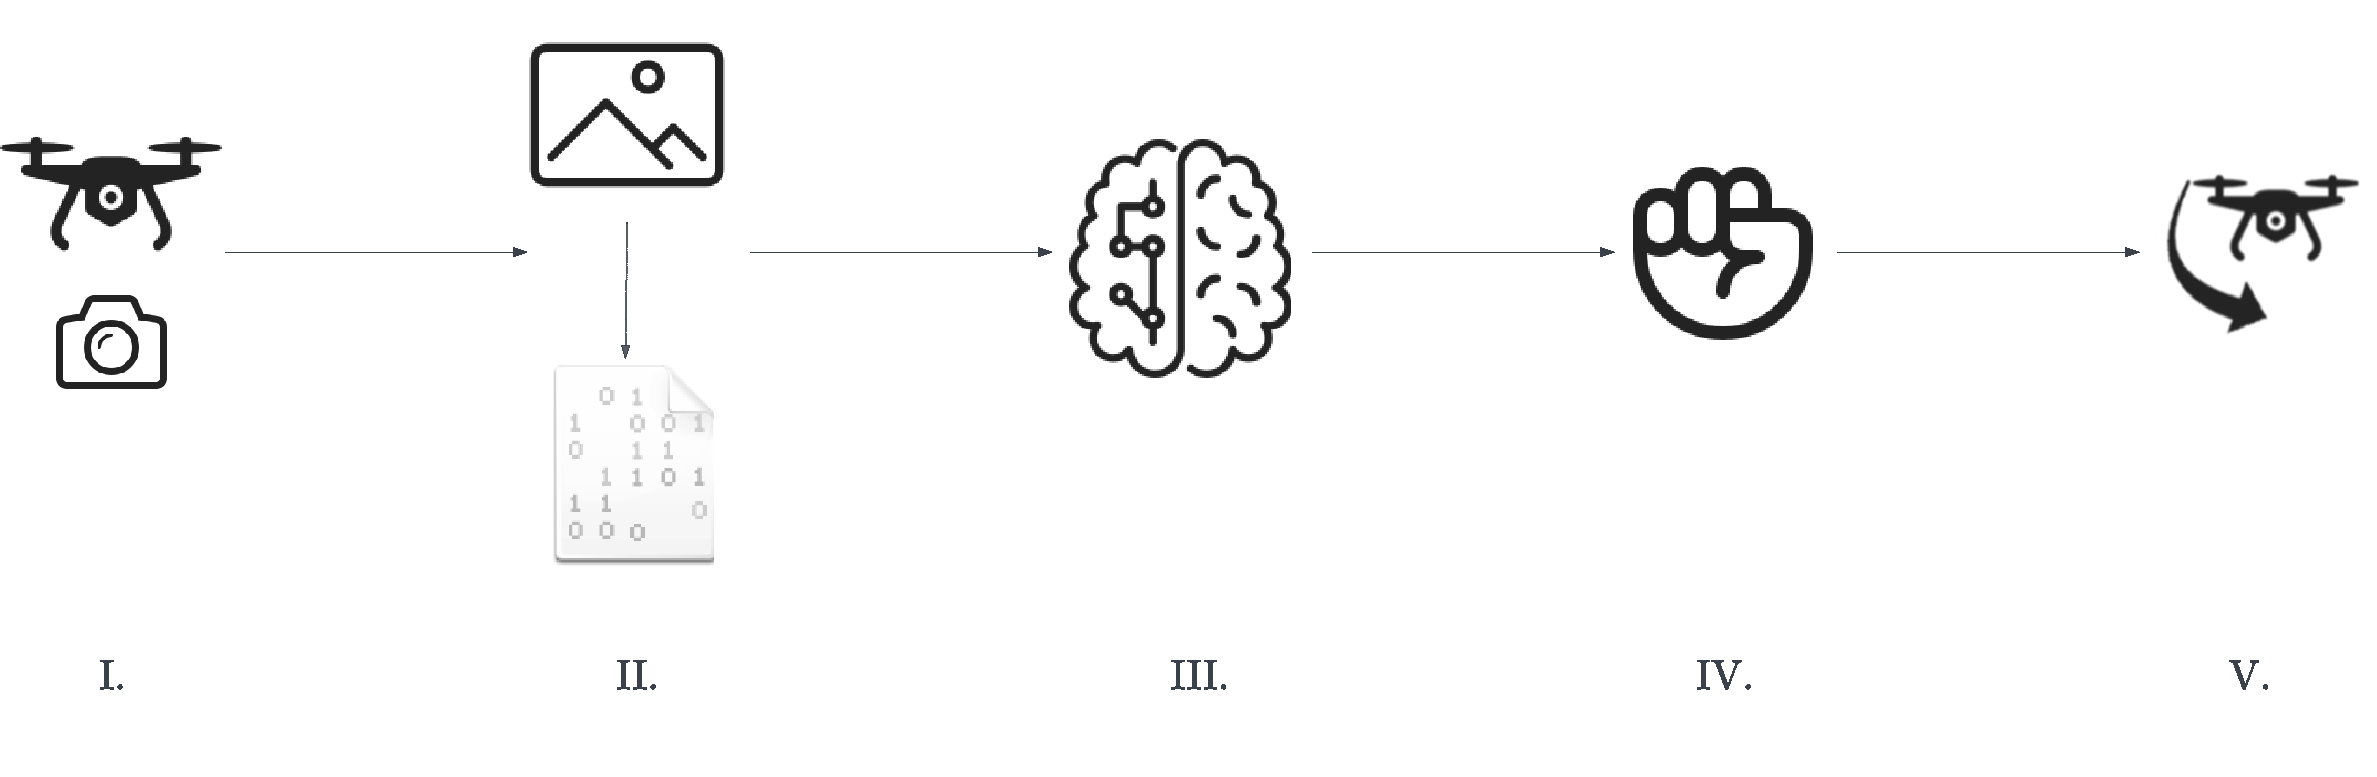
\includegraphics[width =\textwidth]{images/conclusion.pdf}
	\caption{Steps of the process}
	\label{fig:conclusion}
\end{figure}


 The system receives input images from the drone camera connected to the device (our computer). The image is processed, and the gesture is recognized by our model. After~that, the drone executes the corresponding command. 
 The project demonstrates how we can control a drone in an entertaining and educational way while highlighting the potential of gesture recognition technology in various industries and applications.
